\documentclass[a4paper,12pt,french] {article}

\usepackage[sujet]{../../Style}

\fancyhead[L]{Pour le 22/02/2022}
\fancyhead[C]{\textbf{Devoir en temps libre}}
\fancyhead[R]{\seconde 12}

\renewcommand{\baselinestretch}{1.2}

% Passage en A3
%\geometry{a3paper,landscape,bottom=7mm,twocolumn}
%\setlength{\headwidth}{39cm} %42cm-2*margin pour fancyhdr

\begin{document}

Nom: \hfill Prénom: \hfill \

\begin{exercice}
Compléter le tableau suivant:
\begin{center}
\begin{tabularx}{\linewidth}{ 
  | >{\centering\arraybackslash}c 
  | >{\centering\arraybackslash}c
  | >{\centering\arraybackslash}X | }
\hline
Ensemble ou intervalle & Inégalité associée & Représentation\\ \hline 
$\hspace{15mm} \left[ -6;-2 \right[ \hspace{15mm}$ &  & \vspace{5mm} \begin{tikzpicture}[>=latex]
    \node[text=white] at (2,0) {$\textbf{\Big[}$};
    \node[text=white] at (4,0) {$\Big]$};
    \node[below=10pt,text=white] at (2,0) {$a$};
    \node[below=8pt,text=white] at (4,0) {$b$};
    \draw[ultra thick,-,draw=white] (2,0) --(4,0);
    \draw[thick,-,draw=white] (0,0) --(7,0);
\end{tikzpicture}  \\ \hline
 & $\hspace{15mm} 3 < x < 7 \hspace{15mm}$ & \vspace{5mm} \begin{tikzpicture}[>=latex]
    \node[text=white] at (2,0) {$\textbf{\Big[}$};
    \node[text=white] at (4,0) {$\Big]$};
    \node[below=10pt,text=white] at (2,0) {$a$};
    \node[below=8pt,text=white] at (4,0) {$b$};
    \draw[ultra thick,-,draw=white] (2,0) --(4,0);
\end{tikzpicture} \\ \hline
 & & \vspace{5mm} 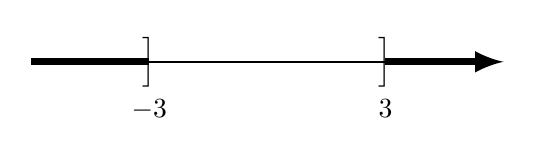
\begin{tikzpicture}[>=latex]
    \draw[thick,-] (0,0) --(5,0);
    \foreach \xp in {0.5,1,...,5.5}{\node[] at (\xp,0) {$\shortmid$};}
    \node[] at (4.5,0) {$\textbf{\Big]}$};
    \node[below=10pt] at (4.5,0) {$3$};
    \draw[line width=2.5pt,->] (4.5,0) --(6,0);
    \node[] at (1.5,0) {$\textbf{\Big]}$};
    \node[below=10pt] at (1.5,0) {$-3$};
    \draw[line width=2.5pt,-] (0,0) --(1.5,0);
\end{tikzpicture} \\ \hline
\end{tabularx}
\end{center}
\end{exercice}

\begin{exercice}
De juin à août, le temps perdu dans les embouteillages à Paris durant les heures de pointe diminue en moyenne de 80\% puis augmente de 272\% en septembre pour atteindre 15 secondes perdues par kilomètre parcouru. Combien de temps est perdu en moyenne par kilomètre par un automobiliste en juin? On pourra utiliser un schéma.

\points 6
\end{exercice}

\begin{exercice}
Soit $f:[0;5] \rightarrow \R$ la fonction qui à $x$ associe $\frac {10x-2}{x+2}$.

\compo[0.7]
{
\begin{enumerate}
\item Compléter le tableau de valeurs suivant, en arrondissant au dixième près:

\begin{center}
\begin{tabularx}{0.9\linewidth}{|c|*{6}{Y|}} \hline
$x$ & $0$ & $1$ & $2$ & $3$ & $4$ & $5$ \\ \hline
$f(x)$ & & & & & & \rule{0pt}{8mm} \\ \hline
\end{tabularx}
\end{center}
\item Tracer sur le repère ci-contre la représentation graphique de $f$.
\item Le point $A(0,5;1,2)$ appartient-il à la courbe de $f$? Justifier par un calcul.

\points 3
\end{enumerate}
}
{
\vspace{-1cm}
\begin{tikzpicture}
\begin{axis}[
styleglobal,
width=\linewidth,
xmin=-0.5, xmax= 5.5,
ymin=-1.5, ymax=7.5,
xtick distance=1,
ytick distance=1,
]

\end{axis}
\end{tikzpicture}
}
\end{exercice}

\begin{exercice} \

\compo[0.4]
{
\begin{center}
\vspace{3mm}
Questions 2 et 3
\begin{tikzpicture}
\begin{axis}[
styleglobal,
width=0.9*\linewidth,
xmin=-2.5, xmax= 6.5,
ymin=-1.5, ymax=4.5,
xtick distance=1,
ytick distance=1,
]
\addplot[styleplot,tension=0.7] plot coordinates {(-2,4) (0,-1) (1,0.5) (2,-1) (4,2) (6,3)} node[pos=0.9,above left] {$\mathscr C_f$}  \pointsextremites;
\end{axis}
\end{tikzpicture}

\vspace{3mm}
Questions 4 et 5
\begin{tikzpicture}
\begin{axis}[
styleglobal,
width=0.9*\linewidth,
xmin=-2.5, xmax= 6.5,
ymin=-1.5, ymax=4.5,
xtick distance=1,
ytick distance=1,
]
\addplot[styleplot,tension=0.7] plot coordinates {(-2,4) (0,-1) (1,0.5) (2,-1) (4,2) (6,3)} node[pos=0.9,above left] {$\mathscr C_f$}  \pointsextremites;
\end{axis}
\end{tikzpicture}
\end{center}
}
{
On a représenté une fonction $f$ sur le repère ci-contre. Des constructions sont demandées pour les questions indiquées.
\begin{enumerate}
\item L'ensemble de définition de $f$ est $\dotfill$
\item L'image de 2 est \dotfill
\item L'image de -1 est \dotfill
\item $1$ a pour antécédent(s) \dotfill
\item $2,5$ possède \makebox[3cm]{\dotfill} antécédent(s).
\item Dresser un tableau de signes de la fonction $f$.
\end{enumerate}
\begin{center}
\begin{tabularx}{0.9\linewidth}{|c|X|} \hline
\rule{0pt}{25pt} & \\ \hline
\phantom{f(x)} & \rule{0pt}{25pt}\\ \hline
\end{tabularx}
\end{center}
}
\end{exercice}

\begin{exercice} \

\compoligne
{
\begin{enumerate}
\item Tracer les droites $d_1$ et $d_2$ d'équations:
$$d_1:y=-2x+3 \ \text{ et } \ d_2:y=\frac 2 3 x+1$$
\end{enumerate}
\begin{centrer}
\begin{tikzpicture}
\begin{axis}[
styleglobal,
width=0.8*\linewidth,
xmin=-2, xmax=4,
ymin=-2, ymax=4,
xtick distance=1,
ytick distance=1,
%major grid style={line width=1pt},
]
\end{axis}
\end{tikzpicture}
\end{centrer}
}
{
\begin{enumerate}[start=2]
\item Déterminer l'équation des droites $d_3$ et $d_4$.
$$\vphantom{\frac 2 3}d_3:y=\hspace{2cm} \text{ et } d_4:y=\hspace{2cm}$$ %vphantom pour l'espacement
\end{enumerate}
\begin{centrer}
\begin{tikzpicture}
\begin{axis}[
styleglobal,
width=0.8*\linewidth,
xmin=-2, xmax=4,
ymin=-2, ymax=4,
xtick distance=1,
ytick distance=1,
%major grid style={line width=1pt},
]
\addplot[styleplot]{3*x-0.5} node[pos=0.55,right] {$d_3$};
\addplot[color=blue,styleplot,densely dotted]{-0.5*x+1} node[pos=0.8,below left] {$d_4$};
\end{axis}
\end{tikzpicture}
\end{centrer}
}
\begin{enumerate}[start=3]
\item En résolvant une équation, déterminer les coordonnées du point d'intersection de $d_1$ et $d_2$.

\points 4
\end{enumerate} 
\end{exercice}

\end{document}

\begin{exercice} \
%%%%% A la base le graphique était vertical, enlever les deux options pour avoir l'original ( il faudra refaire les labels )
\compo[0.38]
{
En utilisant le repère ci-contre:
\begin{enumerate}
\item Tracer deux représentants du vecteur $\vv {AB}$, l'un d'origine $D$, l'autre d'extrémité $C$.
\item Placer $M$, l'image de $C$ par la translation de vecteur $\vv {DB}$.
\item Placer $N$, l'image de $C$ par la translation de vecteur $\vv {DC}$.
\end{enumerate}
}
{
\begin{center}
\vspace{-5mm}
\begin{tikzpicture}[scale=0.48]
\node[draw=none] (liminf) at (0,0) {};
\node[draw=none] (limsup) at (20,15) {};
\draw[step=1,gray,thin] ($(liminf)+(-0.01,-0.01)$) grid ($(limsup)+(0.01,0.01)$);
%\clip (liminf) rectangle (limsup);

%\path [draw=black, line width=2pt] (0,0) -- (-1,-2) -- (0,-4);
%\draw[draw=black, fill = black, fill opacity = 0.3, line width=2pt, even odd rule] 
%        (-4,-8) rectangle (4,-4) (-3,-6.5) rectangle (-1,-5.5) (1,-6.5) rectangle (3,-5.5);
\node[color=black,circle,minimum size=1pt,fill,inner sep=2pt,fill opacity=1,label={180:\textbf{\large A}}] (A) at (2,12) {};
\node[color=black,circle,minimum size=1pt,fill,inner sep=2pt,fill opacity=1,label={180:\textbf{\large B}}] (B) at (9,4) {};
\node[color=black,circle,minimum size=1pt,fill,inner sep=2pt,fill opacity=1,label={-2:\textbf{\large C}}] (C) at (7,8) {};
\node[color=black,circle,minimum size=1pt,fill,inner sep=2pt,fill opacity=1,label={2:\textbf{\large D}}] (D) at (3,3) {};
\draw[line width=1pt,->,>=latex] (16,3) -- ++(2,3) node[pos=0.5,above left] {$\vec u$};
%\node[color=black,circle,minimum size=1pt,fill,inner sep=2pt,fill opacity=1,label={90:\textbf{\large E}}] (E) at (4,-4) {};
%\draw[line width=1pt, shorten <= -10cm, shorten >= -10cm] (A) -- (B);
\end{tikzpicture}
\end{center}
}
\begin{enumerate}
\setcounter{enumi}{3}
\item Comparer les trois caractéristiques des vecteurs $\vec u$ et $\vv {BD}$.

\points 3
\item Quelle est la nature du quadrilatère $BCNM$? Justifier en utilisant des vecteurs:

\points 3
\end{enumerate}

\end{exercice}

\end{document}